\documentclass[10pt]{report}
\usepackage[a4paper,width=150mm,top=25mm,bottom=25mm]{geometry}
\usepackage[utf8]{inputenc}
\usepackage[italian]{babel}
\usepackage{graphicx}
\graphicspath{ {images/} }
\author{Zamboni Marco}
\date{26 Febbraio 2018}
\title{{Computer e Computazione Quantistica}\\
		{\large Liceo Scientifico G.Galilei}}

\usepackage{fancyhdr}
\pagestyle{fancy}

\begin{document}
\documentclass[10pt]{report}
\usepackage[a4paper,width=150mm,top=25mm,bottom=25mm]{geometry}
\usepackage[utf8]{inputenc}
\usepackage[italian]{babel}
\usepackage{graphicx}
\graphicspath{ {images/} }
\begin{document}
    \begin{center}
        \vspace*{1cm}
        
        \Huge
        \textbf{Computer e Computazione quantistica}
        
        \vspace{0.5cm}
		\LARGE        
        (in comparazione a macchine di Turing classiche)
        
        \vspace{1.5cm}
        \huge
        \textbf{Zamboni Marco}
        
        \vfill
        
		
\includegraphics[scale=1]{logoG}\\		
		\vspace{1.0cm}		
		\Large        
        Liceo Scientifico G.Galilei\\
        Italia\\
        26 Febbraio 2018
        
    \end{center}
\end{document}
\tableofcontents
\chapter{Introduzione}
Sono ormai quasi cento anni dall'avvento della fisica moderna e dall'enunciazione delle leggi della meccanica quantistica. Similarmente quasi un secolo è passato dai primi computer e dalla nascita (con Alan Turing) dell'informatica.\\
Non è certamente un caso; infatti l'elettronica e il mondo digitale non esisterebbero senza meccanica quantistica in quanto l'elemento fondamentale, il transistor, è un componente che sfrutta, appunto le leggi quantistiche. In modo molto semplificato si può vedere come un pulsante che può lasciar passare corrente oppure no, che però non funziona meccanicamente aprendo e chiudendo fisicamente un circuito. Esso è infatti azionato da un segnale elettrico che modifica le proprietà quantistiche dei semimetalli con cui è costruito.\\
Senza transistor non si potrebbero gestire i bit [Capitolo 3] nelle memorie flash e soprattutto non si potrebbero creare le porte logiche [Capitolo 4].
Questi computer sono però chiamati comunque classici pur dipendendo dalla meccanica quantistica in quanto l'informazione gestita, cioè i bit, è classica.\\
Si distinguono quindi da essi i computer quantistici che non sfruttano la meccanica quantistica solo come una base necessaria per il funzionamento, bensì fanno in modo che l'informazione manipolata (i qubit) sia essa stessa soggetta alle leggi quantistiche. La ricerca in tale ambito è molto più giovane, ha circa 20 anni, ma ha le potenzialità di apportare miglioramenti e cambiamenti alla società al pari di quello che ha fatto e che sta facendo l'informatica classica.\\
Per questo (e per il mio interesse verso l'informatica e la meccanica quantistica) ho deciso di trattare come argomento personale i Computer e la Computazione quantistica concentrandomi soprattutto sull'opposizione con le macchine di Turing, cioè il modello alla base dei computer classici.
\chapter{Cenni di meccanica quantistica}
\section{Cos'è la meccanica quantistica}
La meccanica quantistica è una teoria fisica che descrive il comportamento della materia, delle radiazioni e delle loro interazioni. In particolare studia i fenomeni microscopici e fa parte del \textit{modello standard} (cioè la teoria fisica che descrive tre delle quattro forze fondamentali: interazioni forte, debole, elettromagnetica e tutte le particelle collegate. Essa è quindi incompatibile solo alla relatività generale che spiega la forza di gravità)

\section{Elementi fondamentali della meccanica quantistica}
\subsection{Dualismo onda-particella}
Nella fisica classica vigevano due blocchi di leggi distinti e apparentemente indipendenti: quelle di Newton, che descrivono i corpi meccanici, e quelle di Maxwell, che invece descrivono i campi elettromagnetici come ad esempio la luce. Quest'ultima era elemento di dibattito in quanto empiricamente con l'esperimento di Young era stato dimostrato che essa è sottoposta ai fenomeni di diffrazione e interferenza: tipici delle onde; ma l'effetto fotoelettrico (emissione di elettroni da parte di una superficie a seguito di un'illuminazione) era spiegabile solo se trattata come insieme di particelle.\\
La meccanica quantistica assume quindi che l'unico modo per spiegare ogni fenomeno fisico è il non limitarsi a considerare la luce \textit{o} onda \textit{o} particella, bensì accettare che essa è entrambi contemporaneamente.\\
Non è comunque solo la luce ad essere soggetta al dualismo, bensì ogni particella: ad esempio nell'esperimento di Zeilinger viene fatto notare come anche i neutroni (normalmente considerati particelle) presentano i fenomeni di interferenza
\subsection{Indeterminazione e casualità}
Per illustrare con miglior chiarezza il concetto partiamo da un paio di esempi.
\subsubsection{Esperimento classico}
Immaginiamo di avere un oggetto, tipo pallina da tennis, che possa essere modellizzato come punto materiale e analizziamo le grandezze fisiche posizione e velocità, ricordandoci che il contesto deve essere controllato in modo che l'esperimento sia ripetibile.\\
All'istante \textit{t=0} la pallina si trova nella posizione \{\textit{x=0,y=0}\} e ad essa imprimiamo una certa velocità. Il moto della pallina sarà parabolico (ricordiamoci che è presente la gravità) come quello mostrato in figura:\\
\begin{center} 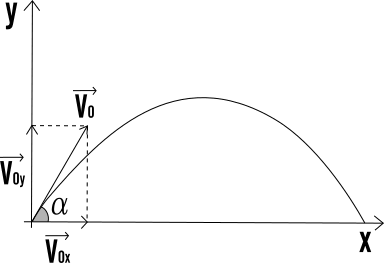
\includegraphics[scale=0.8]{motoParabolico} \end{center}
La cosa fondamentale che vogliamo evincere da questo esperimento è il fatto che ponendoci nelle stesse condizioni: stessa pallina da tennis, stessa posizione all'istante 0 e stessa velocità; il moto sarà sempre identico e la pallina atterrerà sempre nella stessa posizione. Questo ci fa notare come la natura abbia un comportamento deterministico ed è elemento fondamentale del metodo scientifico: se si ottenessero sempre risultati diversi non si potrebbe fare scienza.
\subsubsection{Esperimento quantistico}
Per questo esempio sfruttiamo il già citato esperimento di Zeilinger:
\begin{center} 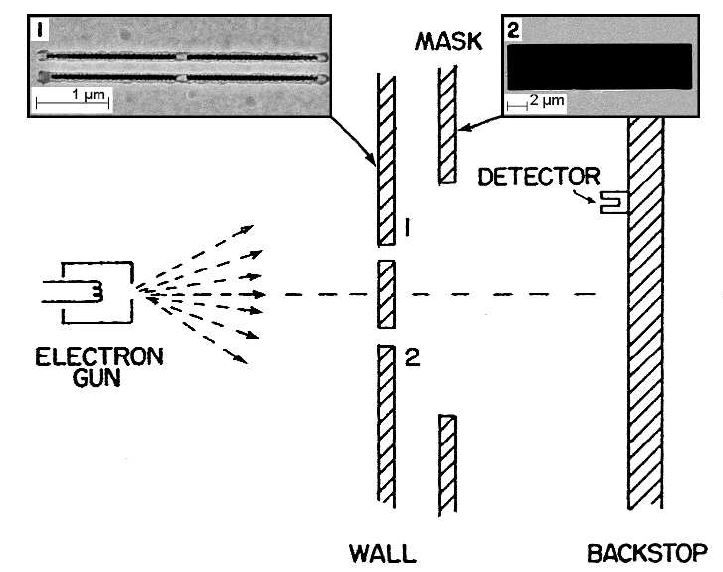
\includegraphics[scale=0.6]{neutronDiffraction} \end{center}
Come si può vedere dall'immagine l'apparato sperimentale è composto da una pistola per neutroni (c'è scritto elettroni, ma il risultato non cambia se si usa una particella oppure l'altra); un muro con due fenditure (che sono dell'ordine di grandezza del diametro della particella), una maschera per evitare al più possibile contaminazioni esterne; un muro finale ove con un detector è possibile trovare la posizione in cui il neutrone è arrivato.
Immaginiamo di esaminare un neutrone per volta; esso è preparato sempre alla stessa maniera e sottoposto sempre allo stesso ambiente; ciò che ci si aspetterebbe, ogni volta misuriamo dove si schianta con il muro finale; compiendo percuò sempre lo stesso identico esperimento quindi ci si aspetterebbe di ottenere sempre lo stesso identico risultato; ma non è così, ogni volta la posizione è diversa.\\
In conclusione non c'è più determinismo, la natura in realtà è casuale e questo è dimostrato empiricamente, quindi non si può più far scienza? Sembrerebbe di no, e sicuramente il percorso del neutrone non è più deterministico e prevedibile con certezza, ma ripetendo l'esperimento un numero molto grande di volte e costruendo un grafico \{numero-neutroni/posizione\} otteniamo un risultato come quello nella figura seguente.
\begin{center} 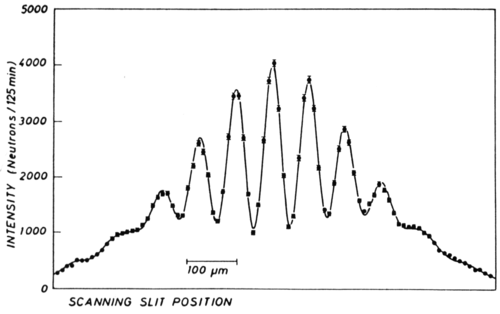
\includegraphics[scale=2.5]{distribuzioneZeilinger} \end{center}
Due sono le osservazioni importanti:
\begin{enumerate}
\item Nel caso in cui si rifacesse tutto da capo otterremmo la stessa identica figura; quindi pur non essendo deterministico un singolo neutrone è possibile fare scienza sulla distribuzione di probabilità di un insieme di essi e quindi descrivere ognuna delle grandezze fisiche di ogni particella come probabilità
\item La figura che si è andata a creare corrisponde esattamente a una figura di interferenza a due fenditure, confermando (come già detto) il dualismo onda-particella
\end{enumerate}
\subsubsection{Limite classico della meccanica quantistica}
A questo punto è necessario chiedersi come mai i modelli matematici applicati a corpi microscopici siano radicalmente diversi da quelli che compongono la fisica classica; in fondo ogni oggetto macroscopico è infine composto da particelle fondamentali che seguono la meccanica quantistica.
Le soluzioni a cui si può arrivare sono molteplici, ma tutte non esaustive, le quali hanno addirittura aperto un dibattito filosofico. Qui però rimaniamo all'interno dell'\textit{interpretazione di Copenaghen}, la più importante. Innanzitutto dato che un corpo macroscopico è formato da un numero enorme di particelle può valere la \textit{legge dei grandi numeri} e quindi ciò che si manifesta non è altro che la "vittoria" dell'evento più probabile. Poi è possibile risalire ad alcune equazione classiche da quelle quantistiche ponendo $\hbar$ $\to$ 0; $\hbar$ è la costante di Planck ridotta, ma non essendo lo scopo dell'elaborato analizzare la matematica dietro la meccanica quantistica l'argomento non verrà approfondito.\\
Il problema che rimane è legato al fenomeno dell'\hyperref[sec:entanglement]{entanglement} che affronteremo fra poco
\subsubsection{Vero stato della materia}
...

\subsection{La sovrapposizione}
Ogni grandezza fisica viene quindi definita e trattata come una distribuzione di probabilità, vediamo cosa un po' più dettagliatemente cosa significa. Come esempio prendiamo lo spin di un elettrone in quanto può assumere solamente due valori: $\frac{1}{2}$ e -$\frac{1}{2}$ al contrario di tante altre che, come ad esempio la posizione, possono assumere infiniti valori continui
\subsubsection{Gli autostati}
Cominciamo a vedere la situazione più semplice: lo spin ha probabilità 1 (o 100\%, è uguale) di essere $\frac{1}{2}$ e probabilità 0 di essere -$\frac{1}{2}$.\\
In questo caso si dice che la grandezza fisica $\textit{spin}$ è in un $\underline{autostato}$ e il valore assunto ($\frac{1}{2}$) è un $\underline{autovalore}$. Quello che accade quindi è che preparando l'esperimento sempre allo stesso l'osservazione dello $\textit{spin}$ produrrà sempre lo stesso risultato.\\
Per estensione qualsiasi grandezza fisica cui la misura di un determinato sistema produce sempre lo stesso risultato (tenendo ovviamente conto degli errori) è un $\underline{autostato}$ indipendentemente da quanti valori la grandezza avrebbe potuto assumere.
\subsubsection{La sovrapposizione}
Quando più valori hanno probabilità non nulla di essere presenti si dice invece che il sistema, per quella grandezza fisica, è in uno stato di $\underline{sovrapposizione}$ (o superposizione dall'inglese $\underline{superposition}$). Ad esempio nel caso la probabilità di ottenere $\frac{1}{2}$ è 0.5 e di -$\frac{1}{2}$ è 0.5 oppure $\frac{1}{2}$: 0.3 e -$\frac{1}{2}$: 0.7 il sistema è in $\underline{sovrapposizione}$. Da ricordare comunque che la somma di tutte le probabilità deve essere sempre 1. Questa però è una semplificazione in quanto in realtà in meccanica quantistica è necessario esprimere le probabilità di ogni valore con numeri complessi rendendo quindi modelli matematici piuttosto complicati, soprattutto in caso di grandezze fisiche continue. A riguardo se ne riparlerà nel capitolo Bit e Qubit nella descrizione di un computer quantistico.\\
Importante ricordare come affermato nell'apposito paragrafico della sotto-sezione precedente che la $\underline{sovrapposizione}$ non esiste in quanto siamo incapaci di preparare in modo preciso l'apparato sperimentale o gli strumenti non sono, ma è un effettivo stato  della materia.\\
Esistono vari modi per produrre uno stato di sovrapposizione con determinate distribuzioni di probabilità in laboratorio, vedremo un esempio nella sezione successiva parlando del principio di Heisenberg
\subsection{La misura}
Nella meccanica quantistica la misura copre un aspetto particolare, piuttosto diverso dalla misura classica.
Infatti in essa è quasi sempre possibile valutare lo stato di un sistema senza perturbarlo negli aspetti interessati; quando non è così la causa sono gli strumenti di misura oppure la perturbazione è determinata e si può risalire matematicamente all'informazione cercata.
In meccanica quantistica invece la misura perturba sempre il sistema e in particolare rompe lo stato di $\underline{sovrapposizione}$ e lo rende un $\underline{autostato}$ con ogni volta un diverso $\underline{autovalore}$ secondo la distribuzione di probabilità.
Questo è molto importante in quanto la trasformazione applicata dalla misura non è prevista dalle varie equazioni (ad esempio quella di Schrodinger) per la trasformazione di un sistema quantistico e non ha una spiegazione logica; diventando quindi il punto di partenza per teorie esotiche come il multimondo (in cui in più universi paralleli si presentano i vari $\underline{autovalori}$
\section{Conseguenze apparentemente controintuitive}
\subsection{Indeterminazione di Heisenberg}
\subsection{Entanglement}
\label{sec:entanglement}
\subsubsection{Il gatto di Schrodinger: vivo o morto?}

\chapter{Conclusione}
\input{chapters/conclusione}
\appendix
\chapter{Appendice}
\section{Bibliografia}
CHINNICI GIORGIO, “Guarda Caso. i meccanismi segreti della meccanica quantistica” - Hoepli (2017)\\
Il libro espone i concetti della meccanica quantistica in una via di mezzo tra il formalismo scientifico e la divulgazione. L’ho usato principalmente nel secondo capitolo della tesina: “Cenni di meccanica quantistica”\\
\section{Sitografia}
https://quantumexperience.ng.bluemix.net/qx/experience\\
Si tratta dell’interfaccia per l’utilizzo di un computer quantistico (situato negli Stati Uniti), e contiene guide all’utilizzo e al concetto generale di computazione quantistica\\
\\
www.youtube.com\\
Vari video di divulgazione a riguardo di computer e computazione quantistica\\
\\
https://github.com/QISKit/qiskit-sdk-py\\
Framework contenente un simulatore di computer quantistico e interprete del linguaggio macchina\\
\\
https://www.dwavesys.com/\\
Sito di una delle maggiori start-up a riguardo dei computer quantistici; presente come vengono costruiti\\
\\
https://www.scottaaronson.com/blog/?p=208\\
Spiegazione dell’algoritmo di Shor a cura di un Scott Aaronson, professore al MIT e  esperto in computazione quantistica
\end{document}
